\documentclass[]{scrartcl}
\usepackage{graphicx}
\usepackage{hyperref}
\usepackage[dvipsnames]{xcolor}
\definecolor{mygray}{gray}{0.9}

% Title Page
\title{\textbf{Parallel computing - Exercise 6}}
\author{Michela Venturini}
\date{Spring 2019}

\begin{document}
\maketitle
\section{Implement the Fast-Transpose Algorithm in CUDA C with shared memory}
 The code implements the fast transpose algorithm in CUDA C and produces a comparison between the performances in both the case by means of the \textit{memory bandwidth}. The implementation is based on the NVIDIA document \hyperlink{mt}{MatrixTranspose} and exploits the benefits gained through the usage of a tile to improve the access memory pattern. The code is executed on Ulysses by using a host node provided with a GPU.
\section{Results}
The image \ref{fig_1} shows the results of the comparison between the Naive algorithm and the improved one. It is straightforward that the performance of the improved algorithm overcomes the base case. We can notice that the peak in terms of bandwidth is the case of 500 threads and the worst that with 1000 threads. 
 \begin{figure}[]
	\begin{centering}
		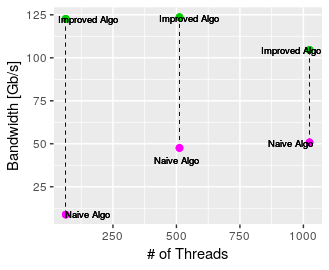
\includegraphics[scale=1]{plot6}
		\caption{Comparison between Naive and Improved implementations}
		\label{fig_1}
	\end{centering}
\end{figure}


\section{References}
\hypertarget{mt}{[1] }http://www.cs.colostate.edu/~cs675/MatrixTranspose.pdf

\end{document} 